	\documentclass[12pt]{article}
	\usepackage{fullpage,amsfonts}
	\usepackage{enumerate}
	\usepackage{amsmath}
	\usepackage{mathtools}
	\usepackage{float}
\usepackage{graphicx} 
\usepackage{caption}
\usepackage{subcaption}
\usepackage[breaklinks]{hyperref}
	
\usepackage{titling}
	\newcommand{\N}{\mathbb{N}}
	\newcommand{\Z}{\mathbb{Z}}
	\newcommand{\Q}{\mathbb{Q}}
	\newcommand{\R}{\mathbb{R}}
	\DeclarePairedDelimiter{\ceil}{\lceil}{\rceil}
	
	\title{\textbf{Spring 2018 CSE534 Final Project Report: A Hybrid implementation of Random Early Detection (RED) and delay-based priority queueing in packet switched networks}}
	\author{\textsc{Abiyaz Chowdhury} \\ \textsc{Rohit Chatterjee}}
	\date{\today}
\begin{document}
\maketitle
\begin{abstract}
This project implements an improvement to the Random Early Detection (RED) algorithm used for mitigating congestion in packet switched networks. Random early detection is based on the notion of dropping packets and marking their congestion bit before the link's ingress/egress buffers (the packet queues) become full. The packets are flagged probalistically, with the probability of doing so being commensurate with the queue size over some period. An improvement to this algorithm is based on the idea of delay-based priority queueing, where priority queues are used instead of FIFO queues. In delay-based priority queueing, the priority metric used for the queues is delay, which is the time in which the packet has been in flight since generation at its origin. Our algorithm implements the naive tail-drop queueing algorithm, the vanilla version of RED, and finally, the improved version of RED that uses priority-based queueing. The algorithm is tested on a variety of virtually simulated networks, and the packet loss and average queue sizes are measured during the process.

\end{abstract}

\section{Introduction}
	One of the main factors that limits the performance of computer networks is network congestion, particularly packet loss which occurs at network links due to overflow of a packet buffer. Packets may be lost in a variety of ways: by being directed to a wrong address, by not being correctly read or accepted and their end destinations, being corrupted or incorrectly split, due to congestion inside the network, all among many other possible reasons. Among these, congestion is often the most pervasive (and pernicious) type of packet loss, and so a great deal of effort goes into minimizing network congestion through various means. This is of course the motivation behind the celebrated congestion control mechanism in TCP, but there are other means to tackle this problem. Notably, TCP congestion control is implemented only at end systems, and therefore does not directly handle local congestion at midpoints or routers - which is really most of the network.

Recall that a router is a device that has multiple connections to other devices on the internet, and its basic function is to forward packets along correct paths to their destination. Thus router function is not immediate, since the router must determine where it must send each packet once it receives it. Further, each connection on the internet has its own capacity or bandwidth which fixes the maximum rate at which packets can be sent along this connection. The upshot of all this is that there is a certain maximum rate at which a given router can despatch incoming packets, and thus if it receives packets at a grater rate then there is congestion at the router. The way this is dealt with is straightforward: the router has a predefined amount of buffer memory to deal with stranded packets, and this is called the queue. The process of managing these packets and using the queue is called queueing. The most natural (and widely used) way to perform queueing is to do it in a first-in-first-out manner: the earliest recieved packet in the  queue is sent out first by the router (hence the term queue), and the queue receives packets as long as packets come in faster than they can be sent out. Once the queue fills up, subsequent incoming packets are all dropped till the queue has space to accept more packets again.

On the face of things, one would not expect anything more from the queueing algorithm; there seems to be no apparent reason why the functioning of the queue should be related to the network performance. In other words, if the network is otherwise well-managed, we might expect such congestion to be short in duration, and therefore assume that the queue absorbs such bursty behaviour and in fact smoothens out traffic heading out from the router. However this is not always the case, and we can see that this method of queue operation may actually hamper network performance in some scenarios. For example, consider the case where multiple flows are present in the network and these flows happen to synchronize in such a manner that only a few flows are always present at the head of the queue, and consequently several other flows have their packets dropped repeatedly. Thus the network only properly services these first few flows, and the other flows in the network receive very little bandwidth. This phenomenon is known as \textit{lockout}. Another undesirable scenario can be brought about by prolonged congestion. If a lot of packets arrive to an already full queue, many packets are dropped simultaneously. This can trigger transport layer level congestion control mechanisms, leading to synchronized responses (back-off) among multiple flows. As a result, the overall load on the network may drop below the capacity of the link and then rise back to exceed the link's capacity resulting in a full queue and so on, giving rise to large oscillations in the network utilization. This oscillating behavior is opposite of the buffer's expected function, which is to also act as a smoothing filter. It also implies inefficient bandwidth usage. This phenomenon is known as \textit{full queue}.

Thus we see that it is not straightforward to manage queueing behaviour with congestion control in mind. Ideally, a good queueing algorithm should be able to identify signs of imminent congestion and high traffic volumes, and take actions to avoid such outcomes. In more concrete terms, the queueing algorithm should manage to keep the average queue size low for the most part, by taking specific actions such as dropping or marking packets (thereby initializing transport level congestion control mechanisms). A low queue size implies that the router can handle and smoothen out bursty traffic, and also that the "queue lag" for any given packet is low: this is the delay the packet faces from just being in the queue till it is sent out. There are various queueing algorithms that try to accomplish this in different ways. In this project, we try to manually run some of these algorithms on a virtual network (using Mininet) and try to analyse their performance and compare the results.

\section{Queuing algorithms}
We discuss three particular queueing algorithms which have been implemented in this project.

\subsection{Tail-drop}
Tail-drop is the most primitive of queue management algorithms. It simply involves dropping packets that arrive at full queues. TCP's congestion control mechanism is designed to react to such packet loss by reducing the congestion window size, so that packet loss is less likely in the future. However, TCP is a reactive algorithm which takes time to respond to changes in the network and under tail-drop, packet loss will usually remain for a while at a full queue until all incoming flows to that queue reduce their congestion window, a process which can take some time. Tail-drop is therefore tardy in its response to congestion, since it does nothing to reduce congestion until the queues become full, at which point packet loss is bound to be high. Another disadvantage behind tail-drop is its failure to accommodate burst traffic. Sometimes, a host may generate a sudden swarm of packets, which under tail-drop will cause the queue to immediately fill up and leading to packet loss. The problem is that tail-drop fails to prematurely react to the swarming packets, which immediately fill up the packet buffer. Random Early Detection (RED) tries to address some of these issues. 
	
\subsection{Random Early Detection (RED)}
Random Early Detection attempts to address some of the issues of tail-drop by prematurely dropping packets. This means that with some probability, incoming packets are dropped even when the queue is not full. The probability of dropping a packet is proportional to the size of the queue. This premature dropping of packets allows the network to inform the sender to throttle its congestion window much sooner than what is done by tail-drop, which is to not do anything until the queue is full, at which point packet loss will be high. Although some packets are dropped early under RED, the overall gain is significant, since it gives the sender more time to react to congestion, potentially preventing overflow at the queue, thereby preventing the huge packet loss that would inevitably occur under tail-drop. In addition, burst traffic is essentially accommodated by the router quickly dropping packets so the sender can throttle the burst and spread the transfer more evenly across time. After all, senders do not know the buffer sizes at the routers and links. Early detection therefore allows routers to quickly inform the senders that congestion avoidance is necessary. 

\subsection{RED with delay-based priority queueing}
Typical queueing algorithms, including RED, do not discriminate between packets in the sense that packets are merely processed on a first-come first-serve basis.. This is true even at the link layer: the first packet to arrive in an ingress interface is switched to its correspondding egress interface when the switch is ready. Neither routers nor switches typically consider packets which have arrived after packets which have yet to be processed. One issue with this is that some packets truly deserve to be processed early, even if they arrived late to a link interface. If these packets are not processed early enough, they may simply become useless when it is finally time for the router to process them. \cite{main_paper} discusses the importance of VoIP packets, and their need to be processed quickly if there is to be minimal jitter in the audio output. One simple, yet effective approach to measuring packet priority is simply using the delay of the packet, which is the time since the packet's inception at its sender. Earlier packets are given more priority, since their tardiness may render them useless at the receiver. Not only does this improve the quality of service for the network as a whole, but it also potentially reduces network congestion, especially for flows where packets that arrive too late are forced to be retransmitted. This is particularly an issue in some time-sensitive applications, particularly feedback control systems which rely on the use of network communications, such as missile guidance control. In these cases, tardy packets are useless at the receiver, and require fast retransmissions which can be immediately responded to at the receiver. It is up to the links to ensure that these packets are delivered on a timely basis, and one such approach is to use delay-based priority queues at the link interfaces. Delay-based priority queues also effectively manage burst traffic, since packets from the same burst flow are likely to have similar priority (delay) values and therefore they will not be favored over earlier packets, even though they are more numerous.

\section{Implementation}
Our implementation is built on the mininet framework, with mininext and quagga used as high-level interfaces to mininet. We had originally considered using OpenFlow to model link interfaces and their queues, but later chose to implement the queueing algorithms from scratch due in part to difficulties faced in using OpenFlow as well as a desire to understand the queueing algorithms at a lower level. Python is used to create the mininet toplogy; Java is used to simulate packet generation and transmission through various mininet topologies, and shell scripts are used to automate these processes. A link to the implementation sources is available at \url{https://github.com/Abi1024/CSE534-Final}. 

\section{Results}
We discuss the performance of the three algorithms discussed under a variety of test scenarios. We will use a simplified unit system where $1$ refers to the upload bandwidth of the first sending host (per millisecond), and all other values are represented relative to this value. 

\subsection{Two hosts connected by a link: burst traffic from one host to the other}
In our first experiment, a simple network with two hosts connected by a link, we simulate a transmission of burst traffic from one host to the other through the link. The sender's upload bandwidth is $1$, the receiver's download bandwidth is also $1$. The link has a rate of $2$, and the link has a single buffer of capacity $5$. Since the link's capacity exceeds the usage by the hosts, we do not expect this simple situation to cause network congestion in the asymptotic case. However, because the traffic is bursty, it is occassionally possible for the queue to become full, resulting in some packet loss. We observe how the queueing algorithms respond
to this simple scenario.

\subsection{Four hosts connected by a link: brust traffic from H1 to H4 and burst traffic from H4 to H1}


   \begin{figure}[H]
    \centering
    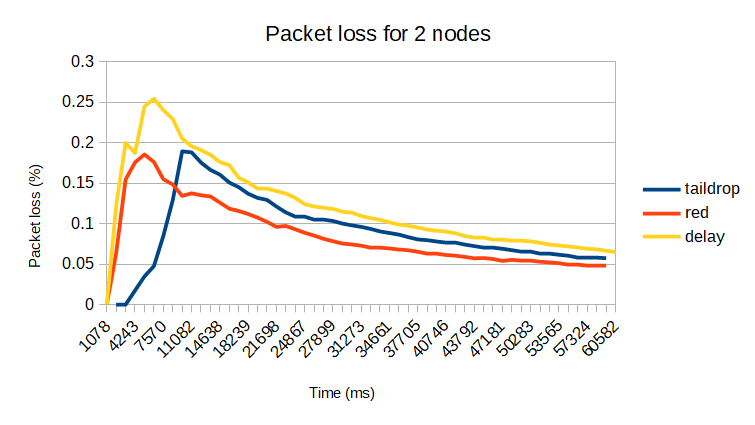
\includegraphics{figure1.png}
    \centering
    \caption{Packet loss for 2 hosts and 1 router}
\end{figure} 

\begin{figure}[H]
    \centering
    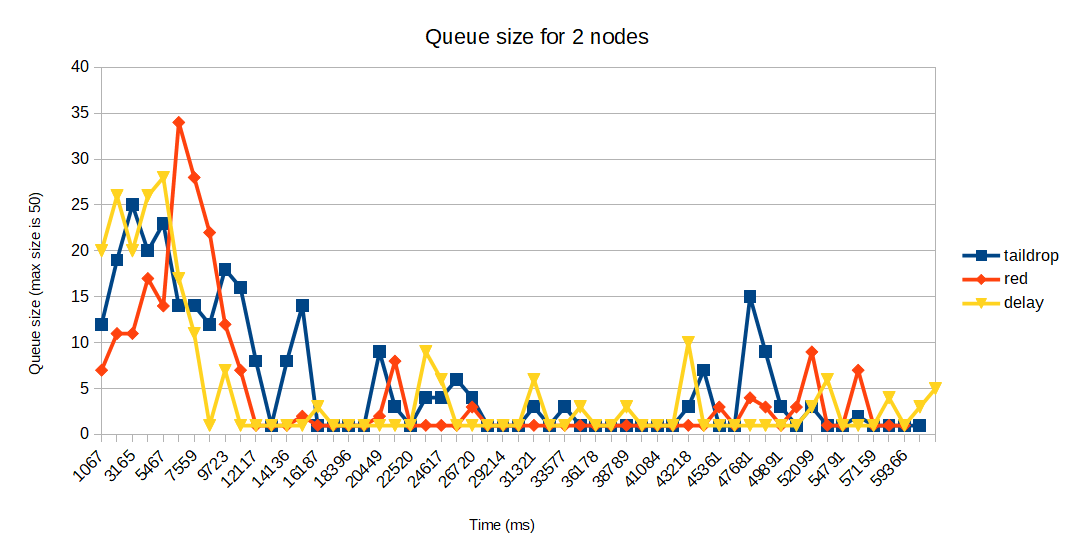
\includegraphics{figure2.png}
    \centering
    \caption{Packet loss for 2 hosts and 1 router}
\end{figure} 

\begin{figure}[H]
    \centering
    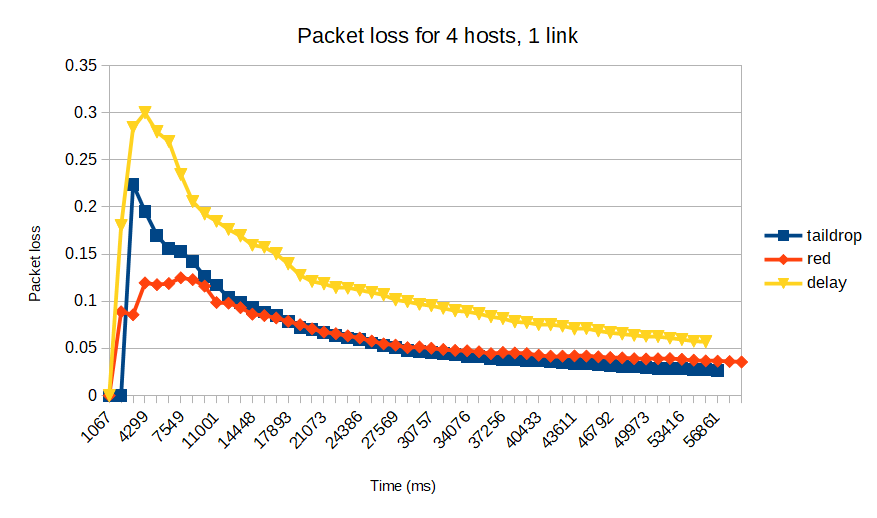
\includegraphics{figure3.png}
    \centering
    \caption{Packet loss for 2 hosts and 1 router}
\end{figure} 

\begin{figure}[H]
    \centering
    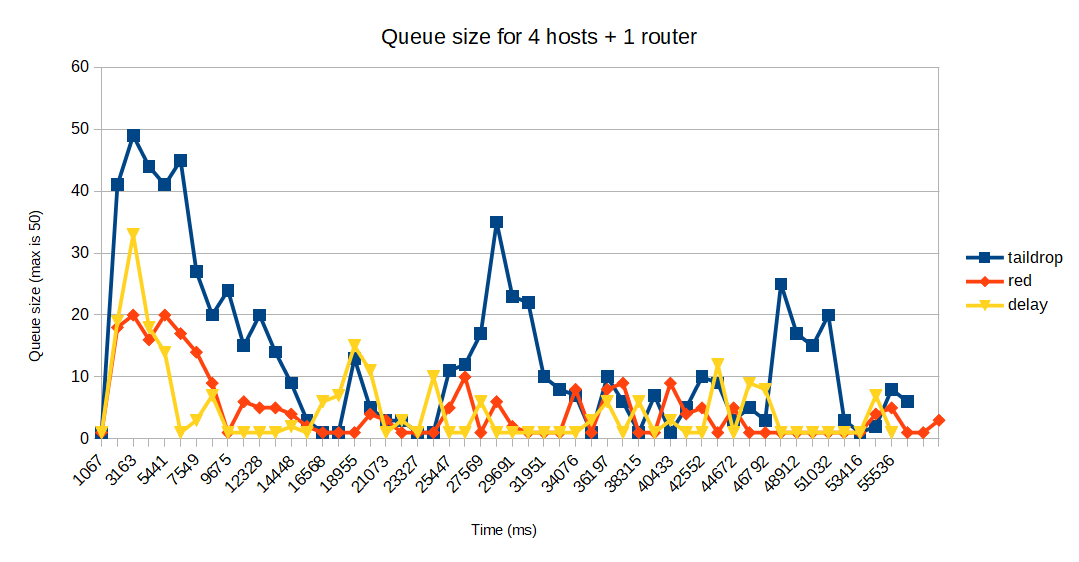
\includegraphics{figure4.png}
    \centering
    \caption{Packet loss for 2 hosts and 1 router}
\end{figure} 
 

\begin{thebibliography}{9}
\bibitem{red_paper}


\bibitem{main_paper}
	Olariu, Cristian, Martin Zuber, and Christina Thorpe. \emph{Delay-based priority queueing for VoIP over Software Defined Networks.} Integrated Network and Service Management (IM), 2017 IFIP/IEEE Symposium on. IEEE, 2017.
\end{thebibliography}

\end{document}
